\chapter{Evaluation}
\label{chap:evaluation}



\section{Experiments}
\label{s:Experiments}
Five experiments were performed to validate the functionality of the tags.
The first two are non specific and ment to test the setup in a stable environment.
Experiments three to five are intended to test the detection of unwanted circumstances.
For all experiments the query-frequency was set to 330s, so measurment was evaluated once every 330s.
The measurements queries are spread across this timeframe.
Each experiment lasted between 40 minutes and one hour.
The results were stored on the phone and then exported using email.
The analysis of the data and creation of graphs was then performed using a Jupiter Notebook, using Pandas and Pyplot for datamanagment and the creation of graphs.



\subsection{Experiment 1: Static}
\label{ss:exp_1}
The four tags where placed on the corners of a 80 cm by 50 cm rectangle on a wooden table.
Each tag was turned on sequentially and given enough time to establish the network.
The phone then was connected to one tag.
The parameters in the app were left unchanged.
The default parameters are large enough, that no measurement should be large enough to trigger a warning.
The setup was then left untouched for 35 min.
The goal of this experiment was, to gauge by how much the measurements can vary in a static environment.


\subsection{Experiment 2: Coordinated movement}
\label{ss:exp_2}

\subsection{Experiment 3: Temperature}
\label{ss:exp_3}
The four tags were placed in the same 80 cm by 50 cm rectangle as in experiment one.
One tag placed on a elevated surface, 4 cm above the table.
Under the tag seven candles were placed (see figure TODO, Bild einfügen).
Next to the tag two thermometers detectors were placed.
Each tag was turned on sequentially and given enough time to establish the network.
The phone then was connected to one tag.
The max Temperature parameter in the app was changed to 35\degree C.
After 20 minutes the candles were lit.
The experiment was then left alone for another 30 minutes.
The independent thermometers were filmed during the process, to allow for later review and comparesment.
The goal of experiment 3 was to test the temperature detection capabilities of the system.


\subsection{Experiment 4: Gyroscope}
\label{ss:exp_4_1}
Again all for tags were placed on a 80 cm by 50 cm rectangle.
Each tag was turned on sequentially and given enough time to establish the network.
The phone then was connected to one tag.
The maximal allowed angular difference was set to 30\degree .
After 20 minutes one tag was turned by 90\degree counterclockwise.
The experiment then ran for another 30 minutes.
The goal of experiment number 4 was to test the detection of unwanted rotations.
Experiment four was repeated with, with the gyro sending the angular velocity for all axes instead of the current position.


\subsection{Experiment 5: Distance}
\label{ss:exp_5}
The same 80 cm by 50 cm rectangle setup was used.
The tags were turned on sequentilay, giving them enough time to build the network.
The phone was connected to one tag.
The max distance parameter was set to 20 centimeter.
After 20 minutes, one tag was moved parallel to the shorter rectangle line about 20 cm towards the tag on the next corner.
The system was then left resting for another 30 minutes.
The goal of experiment number 5 was to test the detection of unwanted movement.

\section{Experiment Results}
\label{s:exp_res}

In this section the results of the experiments are presented.
All eperiments were performed two to three times.
In each section only the data-set from the first experiment run is presented fully.
The other experiments will be mentioned only, if they have differing data or to confrim an unexpected datapoint.

\subsection{Experiment 1: Static}
\label{ss:exp_1_result}
In eperiment one, all measurements are expected to be unchanging.
Table \ref{t:exp1_means} shows the mean values for temperature, humidity and angle during the experiment by tag.
Figures \ref{f:exp1_graphs_temp}, \ref{f:exp1_graphs_hum}, \ref{f:exp1_graphs_gyro}, \ref{f:exp1_graphs_dist} shows the change of these values over time.

\begin{table}[h!]
	\centering
	\begin{tabular}{|c|c|c|}
		\hline
		\textbf{Tag} & \textbf{Temp Mean} & \textbf{Hum Mean} \\
		\hline
		1 & 22.06 & 32.56 \\
		2 & 21.90 & 33.93 \\
		3 & 22.06 & 32.94 \\
		4 & 21.87 & 32.80 \\
		\hline
	\end{tabular}
	\caption{Mean and Variances for Temperature, Humidity, and Gyroscope Data by Tag during experiment 1}
	\label{t:exp1_means}
\end{table}

\begin{figure}[ht!]
	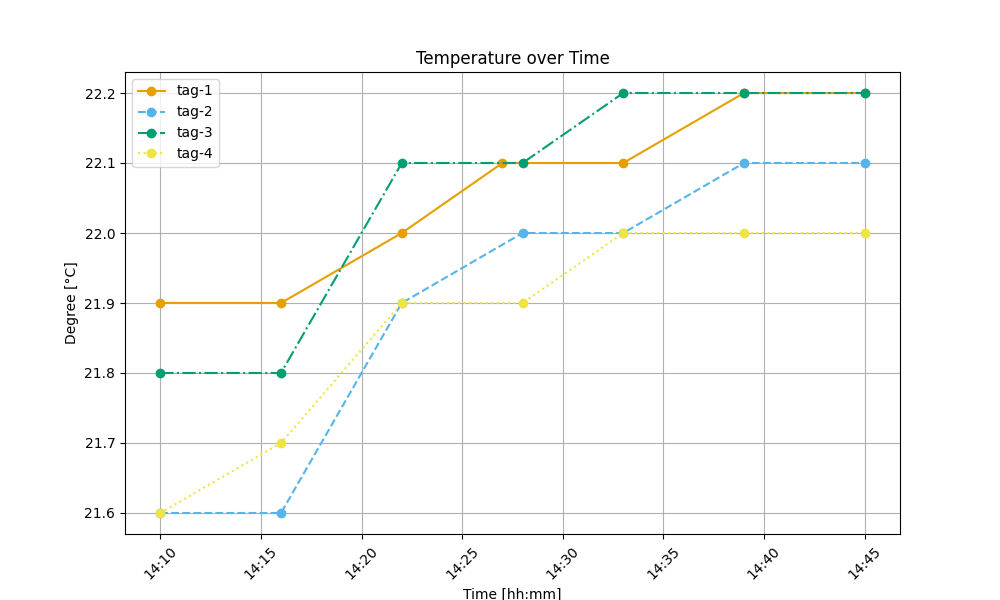
\includegraphics[width=\linewidth]{graphics/exp/exp1_temp_plot_0.png}
	\caption{Experiment 1, temperature over time.}
	\label{f:exp1_graphs_temp}
\end{figure}


All four tags have a similar mean temperature and are all less than 0.2 \degree C apart from each other.
The varaince are also small, tag two having the highest one with 0.05 \degree C variance. 
The graph shows that all tags have a rising temperature.
The increase is quite small with tag two having the biggest increase of 0.5 \degree C over 20 minutes.
When the experiment was repeated, the means stayed similar and the variance small, but the temperature changed course.
A downward trend was visible, instead of the upward trend seen during the first experiment.

\begin{figure}[ht!]
	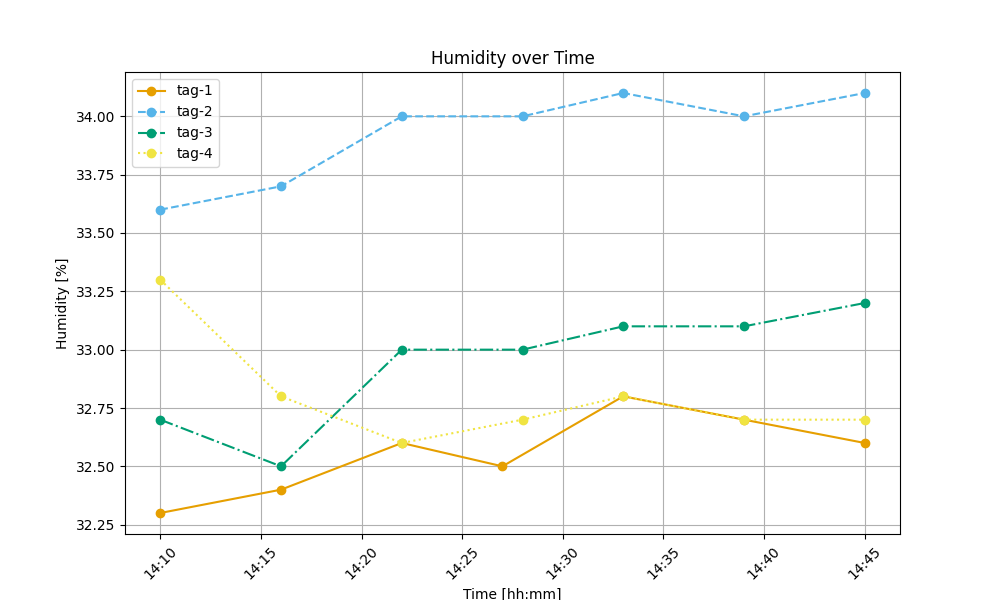
\includegraphics[width=\linewidth]{graphics/exp/exp1_hum_plot_0.png}
	\caption{Experiment 1, humidty over time.}
	\label{f:exp1_graphs_hum}
\end{figure}

Humidity follows a similar trajectory as.
The means only vary by 1.5 \% pt.
The variance is small, with tag three having the biggest variance with 0.06\% pt.
During the first experiment, humidity increased by a small amount.
When the experiment was repeated, the humidity dropped during the experiment.


\begin{figure}[ht!]
	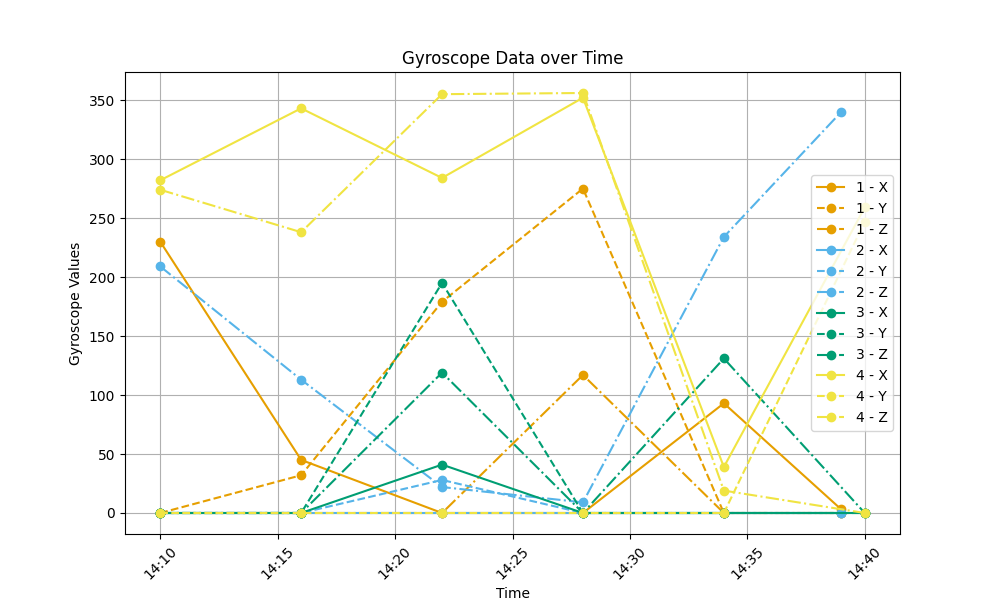
\includegraphics[width=\linewidth]{graphics/exp/exp1_gyro_data_plot_0.png}
	\caption{Experiment 1, angles over time.}
	\label{f:exp1_graphs_gyro}
\end{figure}

Since all tags were stationary during the experiment, the gyro sensor was expected to be unchanging.
This is not what happened.
looking at the graph \ref{f:exp1_graphs_gyro} it is clear, that the measurement shows a wide range of angles for each tag and axis.
The only exception is tag 2 around the x axis, which stays at 0 for the whole measurement duration.
Since angle measurements fall into modular arithmetic, it "wrappes around" at 360\degree , means can only meanigfully be taken if the angles are in a small range.
Since this is not the case for most tags, the only thing that can be said is, that tag 2 has a mean of 0 with variance 0 around axis x.


\begin{figure}[ht!]
	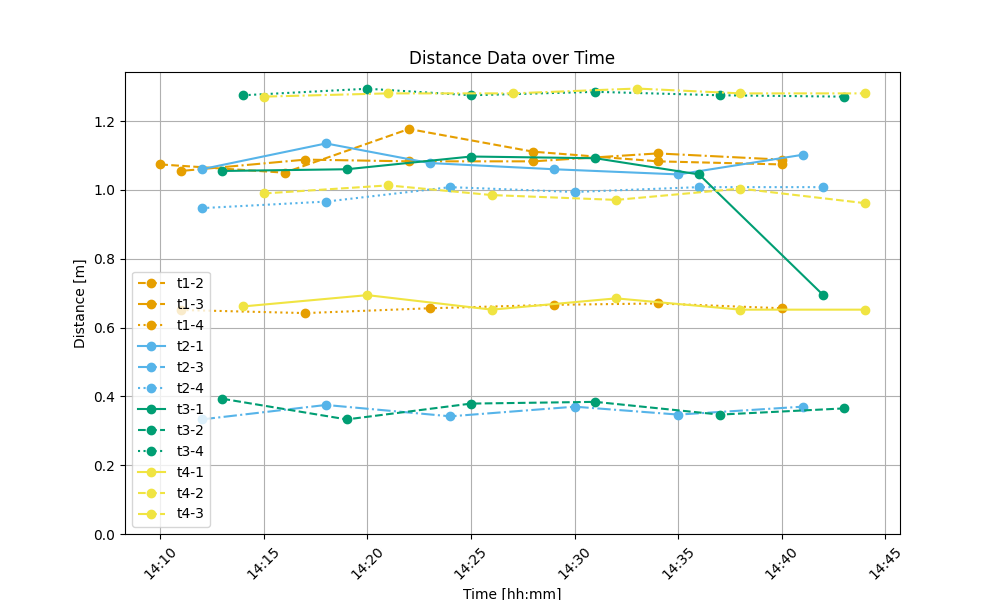
\includegraphics[width=\linewidth]{graphics/exp/exp1_dist_data_plot_0.png}
	\caption{Experiment 1, distance over time.}
	\label{f:exp1_graphs_dist}
\end{figure}

Table \ref{t:exp1_means}, shows the mean of the measured distances, the row entry beeing the queried tag that initiates the distance measurement, and the row corresponding to the responding tag.
By looking to the measurements diagonaly oposed to each other, one can see that the measured distaances is the the same, indipendent of who initiated the measurement, up to a range of two centimeters.
The varince on table \ref{t:exp1_dist_var} also show, that these measurements are stable over time and don't change by much.
Looking at the graphs on figure \ref{f:exp1_graphs_dist}, the pairs of measurements are visible.
One outlier happens when tag 3 measures the distance to tag 1 at very end of the measurements.
When repearing the measurements these outliers happened again, a bit less frequently then twice per hour.
The outliers always affected a measurement involving tag 1.
The distances measured do not correspond to the actual distances the tags had to each other, also seen in table \ref{t:exp1_dist_means}.
The measured distances can be as far of as 0.5 meters.
The two larger distances, 0.8 and 0.94 meters, correspond to the two larger measured values for each tag, while the smallest measured value always corresponds to the smallest distance, 0.5 meters.
The two larger values are not always ordered correctly, 0.94 meters sometimes beeing measured smaller then 0.8 meters.
In repeated experiments, all these facts stayed true.

\begin{table}[h!]
	\centering
	\begin{tabular}{|c|c c c c|}
		\hline
		& \textbf{1} & \textbf{2} & \textbf{3} & \textbf{4} \\
		\hline
		\textbf{1} & 0.0 & 1.094 & 1.084 & 0.657 \\
		\textbf{2} & 1.080 & 0.0 & 0.356 & 0.989 \\
		\textbf{3} & 1.007 & 0.367 & 0.0 & 1.279 \\
		\textbf{4} & 0.666 & 0.987 & 1.281 & 0.0 \\
		\hline
	\end{tabular}
	\begin{tabular}{|c|c c c c|}
		\hline
		& \textbf{1} & \textbf{2} & \textbf{3} & \textbf{4} \\
		\hline
		\textbf{1} & 0.0 & 0.8 & 0.94 & 0.5 \\
		\textbf{2} & 0.8 & 0.0 & 0.5 & 0.94 \\
		\textbf{3} & 0.94 & 0.5 & 0.0 & 0.8 \\
		\textbf{4} & 0.5 & 0.94 & 0.8 & 0.0 \\
		\hline
	\end{tabular}
	\caption{Left: Mean distances between tags in experiment 1. Right: Expected values.}
	\label{t:exp1_dist_means}
\end{table}

\begin{table}[h!]
	\centering
	\begin{tabular}{|c|c c c c|}
		\hline
		& \textbf{1} & \textbf{2} & \textbf{3} & \textbf{4} \\
		\hline
		\textbf{1} & 0.0 & 0.002 & 0.000 & 0.000 \\
		\textbf{2} & 0.001 & 0.0 & 0.000 & 0.001 \\
		\textbf{3} & 0.024 & 0.001 & 0.0 & 0.000 \\
		\textbf{4} & 0.000 & 0.000 & 0.000 & 0.0 \\
		\hline
	\end{tabular}
	\caption{Variance of distances between tags in experiment 1. Row corresponds to queried tag.}
	\label{t:exp1_dist_var}
\end{table}

\subsection{Experiment 3: Temperature}
\label{ss:exp_3_result}
Experiment 3 introduced heat-sources the system.
Since the main setup was the same as experiment 1 \ref{ss:exp_1_result}, many of the findings are the same.
In this section, only differences in results are discussed.
If a metric is not measioned, one can assume it behaved the same as for experiment 1  (see section \ref{ss:exp_1_result}).

\begin{figure}[ht!]
	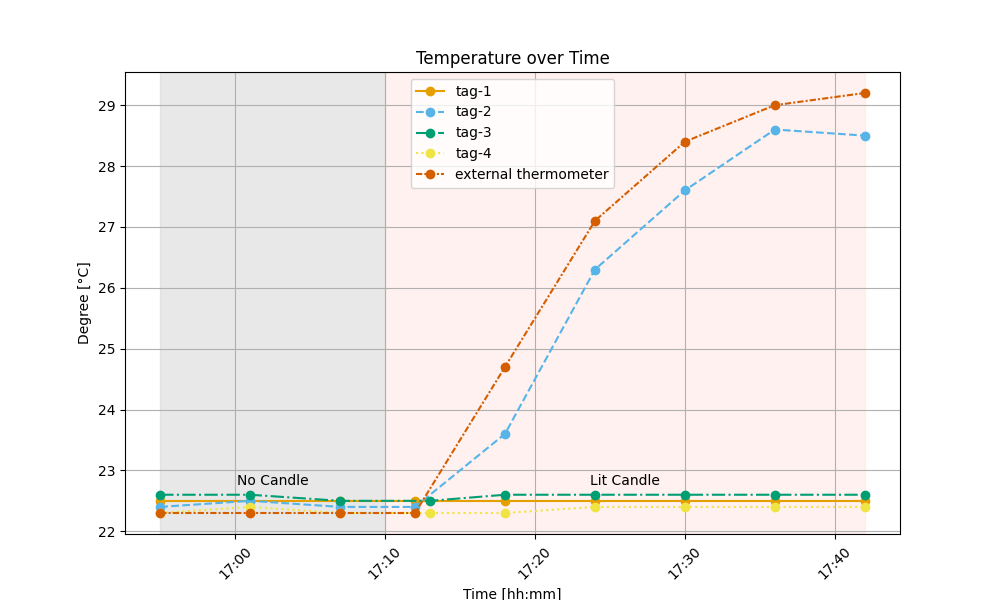
\includegraphics[width=\linewidth]{graphics/exp/exp3_temp_plot_1.png}
	\caption{Experiment 3, temperature over time, mith external measurement added.}
	\label{f:exp3_graphs_temp}
\end{figure}

The progression of the external thermoeter and the internal temperature sensor can be seen in figure \ref{f:exp3_graphs}.
The candles, that functioned as the heat source, were lit at 15.10.
During the next measurement of tag 2, at 15.12, both the external thermoeter and the temperature sensor on tag 2 had not yet registered any change, remaing at 22.4 \degree C.
The extrenal thermometer started rising 1 minutes later, at 15.13.
During the next measurement at 15.18, the temperature-sensor registered a slightly increased temperature of 23.6 \degree C, while the external thermometer registered 24.7 \degree C.
During the next measurement at 17.24 the tag reported 26.3 \degree C while the thermometer showed 27.1 \degree C. 
The measured temperature of the external thermometer keeps klimbing faster than the internal temperature sensor, until the end of the experiment, as seen in Figure \ref{f:exp3_graphs_temp}.
Their distance nether exeeds 1 \degree C and gets smaller towards the end of the experiment.
The other tags do not report any significant change in temperature.

\begin{figure}[ht!]
	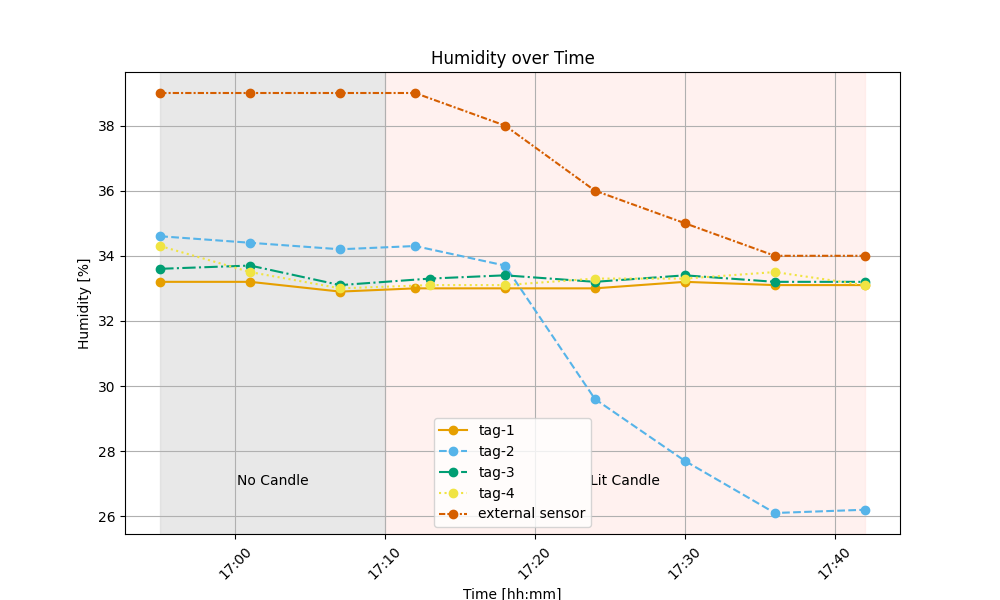
\includegraphics[width=\linewidth]{graphics/exp/exp3_hum_plot_1.png}
	\caption{Experiment 3, humidity over time, with external measurement added.}
	\label{f:exp3_graphs_hum}
\end{figure}


Experiment 3 was intended to test the temperature and not the humidity.
Luckily, the external thermoeter also included a humidity sensor, that could retroactivly be used for evaluation.
Figure \ref{f:exp3_graphs_hum} shows the humidity over time, with a added humidity sensor added to the graph.
Since the external humidity sensor was initialy not intended to be used, it is not perticulalry precise and does not display any digits after the decimal point.
The humidity sensor consitently shows a much higher humidity than the one on the tag.
Once the experiment starts at 15.10, the humidity behaves inversly to the temperature and starts falling.
This happens with the external sensor as well as the internal one in parallel.
The registered values plato at 34\% for the external and 26\% for the internal sensor.
The other tags do not report any significant change in humidity.

\subsection{Experiment 4: Gyroscope}
\label{ss:exp_4_result}

Experiment 4 was intended to check the functionality of the gyroscope.
Temperature and humidity behaviour was the same as in the static experiment \ref{ss:exp_1_result}.
As already seen in during the evaluation of experiment 1, the gyroscope does not work as planned.
Figure \ref{f:exp4_graphs_gyro} shows the values of the gyro over time.
Tag 1 was rotated by 90\degree  at 22.25 around the Z axis.
Their is no disernable change in the output of the gyro during or after this process.

\begin{figure}[ht!]
	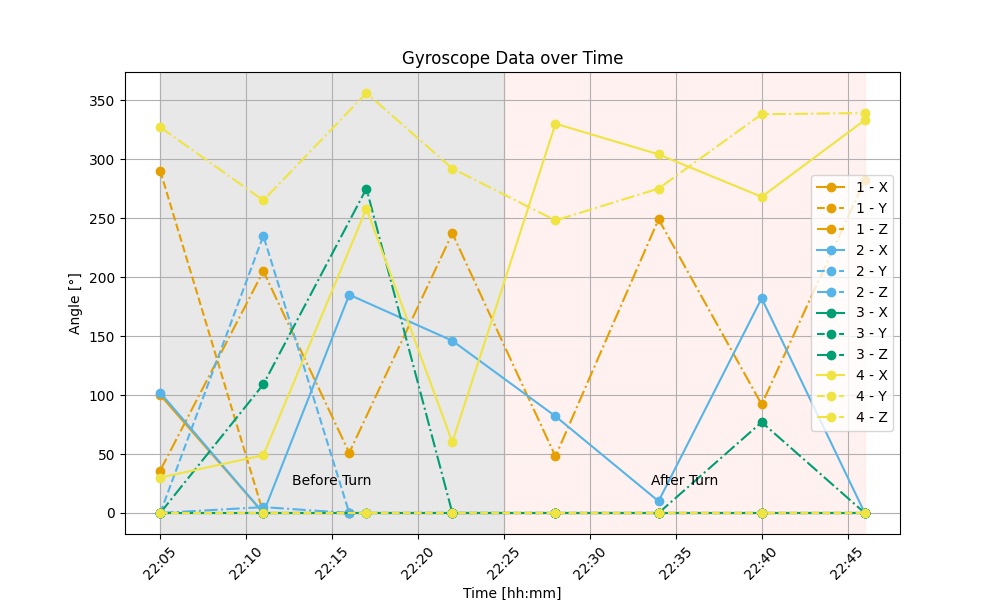
\includegraphics[width=\linewidth]{graphics/exp/exp4_gyro_data_plot_1.png}
	\caption{Experiment 4, gyroscope over time.}
	\label{f:exp4_graphs_gyro}
\end{figure}


Figure \ref{f:exp4_graphs_dist} shows the distances of the tags during the experiment.
Before the event, all tags are in a stable state.
As in experiment 1 \ref{ss:exp_1_result} the distances do not represent what is physically happening.
After the tag is turned at 22.26, all measurements involving tag 1 change, and becomming stable again afterwards.
This can be bit hard to see, since "2-1" and "3-1" have an outlier measurement right before and "1-2" right after.
Distance 1 to 2 and 1 to 3 changes between 0.2 and 0.3 meters and distance 1 to 4 changes by arround 0.4 dm.

\begin{figure}[ht!]
	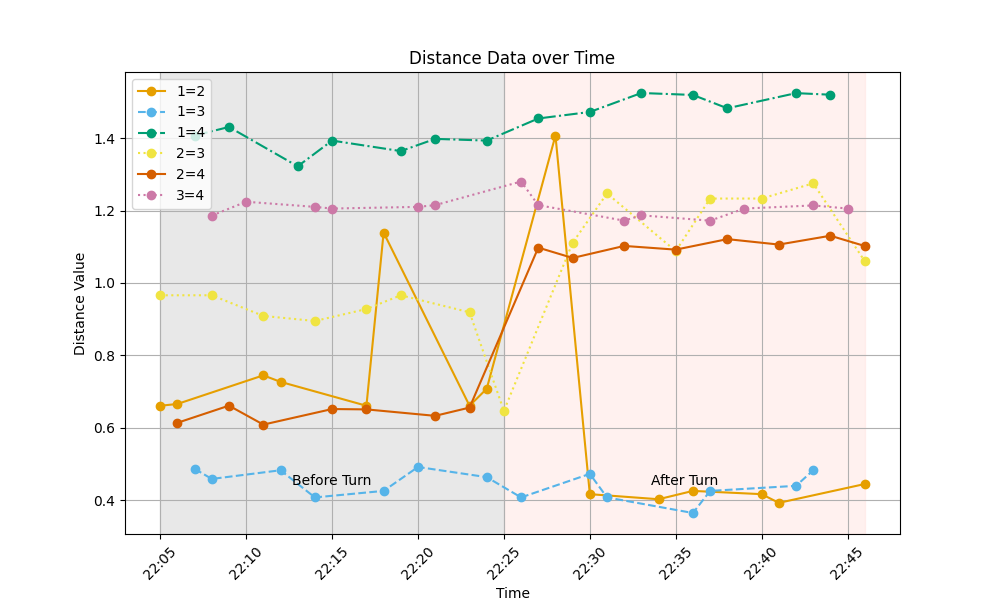
\includegraphics[width=\linewidth]{graphics/exp/exp4_dist_data_plot_1.png}
	\caption{Experiment 4, gyroscope over time.}
	\label{f:exp4_graphs_dist}
\end{figure}


\subsection{Experiment 5: Distance}
\label{ss:exp_3_result}

Experiment 5 was intended to test the distance measurement capabilities of the setup.
Temperature and humidity and gyro behave as they do in experiment 1 \ref{ss:exp_1_result}.
They will not be discussed for this experiment.

\begin{figure}[ht!]
	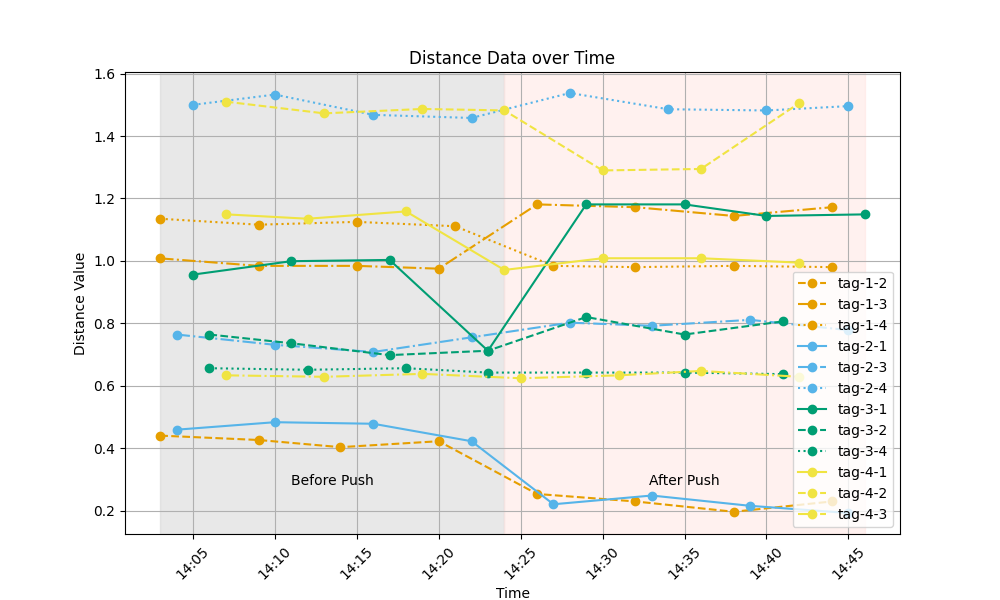
\includegraphics[width=\linewidth]{graphics/exp/exp5_dist_data_plot_2.png}
	\caption{Experiment 5, distance over time.}
	\label{f:exp5_graphs_dist}
\end{figure}

Figure \ref{f:exp5_graphs_dist} shows the measured distances of the 4 tags over time.
As in the static experiment, the measured distances of two devices are similar and mostly stable, before any movement is introduced.
As in experiment 1 the values reported are not correct.
At 14.24 tag 1 is moved by 0.23 meters toward tag 2.
The measured distances to tag 3 increases while the distance to tags 2 and 4 dicreases.
This represent what is happening in reality, since tag 1 is now closer to tag 2 and 4 and further away from tag 3 as before.
The difference in distance is roughly 0.2 meters for tag 2.
This is correct, since tag 1 was moved about that distance towards tag 2.
The measurements show tag 4 now 0.15 meters closer to tag 1.
The effect on tag 4 should be notissable but not as large as it is.
Since the tag moves lateraly towards tag 4, the difference should only be 0.11 meters.
The same is true for tag 3.
The difference in measured distance between 1 and 3 is between 0.15 and 0.2 meters. 
This is too large for the difference a latteral move, it should only be a 0.02 meters difference.
Their is also a small increase in the distance between tags 2 and 3, but which starts before tag 1 was moved.


